\documentclass[12pt]{article}


% \usepackage[authoryear]{natbib}
% \usepackage{amsmath}
% \usepackage{hyperref}
% \usepackage{hyperref}
% \usepackage{geometry}
% \usepackage{graphicx}
% \usepackage{amsfonts}

\input{../../paperProduction/occBind/docs/AMArepresentationNewCmds}



\author{Gary S. Anderson\thanks{The analysis and conclusions set forth are those of the author and do not indicate concurrence by other members of the research staff or the Board of Governors. I would like to thank Luca Guerrieri, Christopher Gust, Hess Chung, Benjamin Johannsen  and Robert Tetlow for their comments and suggestions.  And special thanks to Luca Guerrieri for first noticing that the series representation formulation could lead to an error bound for model solutions.. Any remaining errors are mine alone.}}

\title{A New Series Representation for 
Nonlinear Dynamic Stochastic Model Solutions: General Error Bounds and a New Solution Algorithm}

\date{\today: \currenttime}
\begin{document}

\maketitle

\begin{abstract}
This paper proposes a new series representation for bounded time series paths and uses this representation to construct error bounds for proposed solutions for a very broad class of dynamic stochastic models.
% This error bound calculation accounts for the impact of errors in any of the equations in the system.
The bounds apply for assessing the accuracy of any
proposed model solution regardless of the source.
Consequently, the approach can provide information about the accuracy of perturbation solutions and along with global information to improve them.


The paper also proposes a new algorithm for solving models.
The series representation makes it possible to reliably improve upon an initial
guess for a stochastic model solution by solving a 
potentially complicated, but deterministic problem in the initial time period.
Like the error bound formula, the algorithm is appropriate for models with occasionally binding constraints and/or regime switching. 


The  paper uses a particular implementation of the algorithm to
demonstrate how to use the 
series representation in conjunction with 
Smolyak polynomial function approximation to avoid repeated numerical integration
and to exploit the high degree of parallelism available in the algorithm.







\end{abstract}

\newpage
\tableofcontents
\newpage

\section{Introduction}





Stochastic dynamic non linear economic
models increasingly embody  occasionally binding constraints (OBC).
Since \cite{Christiano2000} a host of
authors have described a variety of approaches. 
\cite{holden15:_exist_dsge,guerrieri15:_occbin,benigno09,hintermaier10,brumm10,nakov08,haefke98,nakata12,gordon11,billi11,Hintermaier2010,Guerrieri2015}


The framework provides a new way to bound the error one can expect from
employing a given proposed model solution and leads to an
algorithm with  components similar to parameterized expectations that
one can use to improve proposed solutions. The series representation makes
it possible to organize the calculation around computing a deterministic
problem at time t given a proposed solution.  The deterministic solution
can accommodate inequality constraints or alternative regimes to produce a
solution for each set of initial conditions.  One can typically arrange,
perhaps by adding auxiliary variables, to produce a ``decision rule''
that one can use to correctly precompute a deterministic conditional
expectation function that can be iterated forward and serves to
improve upon the original proposed solution.
Time invariant stochastic functions 
lead naturally to an associated family of deterministic maps
which can be conveniently represented by the series representation.
Others have also studied error bounds for dynamic stochastic models.\cite{judd2017lower,santos2005accuracy,Santos2000accuracy}

The analysis develops a new series representation for bounded time series.  The author has found no comparable use of a linear reference dynamical system 
used to generate a transformation of one infinite dimensional series into another.\footnote{The algorithms described \cite{holden15:_exist_dsge} and \cite{guerrieri15:_occbin} also exploit the use of ``anticipated shocks'', but do not use the comprehensive formula employed here. }

The paper studies a very general class of models whose 
solutions are characterized by $\eqnFuncSys$, a 
 exhaustive and mutually exclusive set of
of   model equations, $\eqnFunc_i$,  and Boolean valued gates, $\gate_i$. 
that together determine the solution  $x_t\tArg$
%\begin{gather}
%\intertext{ where, each }
%\eqnFuncSysI{i}\equiv \eqnFuncSysIExpl{i} \label{eqnGates}
%\end{gather}
The paper shows how to write down a series representation for any proposed
model solution and to characterize the series representation for a typically
unknown solution in such a way that one can use the model equation Euler errors to construct an error bound for the norm of the distance between the proposed and the exact solution.  This work complements the analysis provided in
\cite{judd2017lower,peralta-alva14,santos2005accuracy,Santos2000accuracy}. 
The paper exploits a formula developed in \citep{anderson10} to provide a
series representation for any time invariant discrete map and its
conditional expectation function:
    \begin{gather*}
      	 x\tArg =B x_{t-1}+ \phi \psi_\epsilon\epsilon + (I - F)^{-1} \phi \psi_c + \sum_{\sForSum=0}^\infty F^\sForSum \phi \ZWOarg(\expct{x_{t+\nu}})\\ \intertext{ so that}
\expct{ x_{t+1}\tArg} =B x\tArg  + (I - F)^{-1} \phi \psi_c+ \sum_{\sForSum =1}^\infty F^{\sForSum-1} \phi \ZWOarg(\expct{x_{t+\nu}}) 
    \end{gather*}
 If these functions satisfy the model equations they provide a solution to for the model. The paper shows how to use the model equation Euler errors to 
 improve the solution.
The paper builds upon and complements the work of
\cite{Judd2014,juddGSSA2011,holden15:_exist_dsge,guerrieri15:_occbin}
In particular it uses
the an-isotropic Smolyak Method and adaptive paralletope method\cite{Judd2014}
and precomputes all integrals required for the conditional expectations.
The algorithm should scale well to large models as many 
of the algorithms components cab be computed in parallel.









Section \ref{sec:newseries} presents a useful new series representation for any bounded time series.
Section \ref{sec:extToMaps} shows how to apply this series representation to time invariant maps.
Section \ref{sec:solnerrorbounds} provides formulas for computing dynamic stochastic model error bounds for proposed  solutions.
Section \ref{sec:algoforsoln} presents a new solution algorithm.
Section \ref{sec:future} discusses directions for future work.
Section \ref{sec:conc} concludes.

\section{A New Series Representation For  Bounded Time Series}
\label{sec:newseries}

\subsection{Linear Reference Models and a Formula for  ``Anticipated Shocks''}
\label{sec:linref}




For any linear homogeneous 
$L$ dimensional 
deterministic 
system 
\begin{gather}
  	 H_{-1} x_{t-1} + H_0 x_t + H_1 x_{t+1}=0\label{hSystem}
\end{gather}
that produces  a unique stable solution, 
it is well known\ \citep{anderson10} that  inhomogeneous solutions 
\begin{gather}
	 H_{-1} x_{t-1} + H_0 x_t + H_1 x_{t+1}=\psi_\epsilon \epsilon +\psi_{c}
\intertext{ can be computed as}
x_t=B x_{t-1} + \phi \psi_\epsilon \epsilon + (I - F)^{-1} \phi \psi_c
\intertext{where}
\phi= (H_0 +H_1 B)^{-1}  \text{ and } \,\,F=-\phi H_1 
\end{gather}
It will be useful to collect the components of this representation for use in
subsequent sections of the paper.
Define $\linMod \equiv \linModMats$.




\begin{theorem}
Consider an arbitrary, but bounded path
 \begin{gather}
   \xWOarg_t \in{R^L}\,\text{ with }\,\infNorm{\xWOarg_t}  \le \bar{\mathcal{X}}\,\,\,\,\,\forall t> 0 \label{aBPath}.
 \end{gather}

Now, given the trajectories \refeq{aBPath}, define 
$  z_{t}$ as  
\begin{gather}
  z_{t} \equiv H_{-1} \xWOarg_{t-1} +  H_0 \xWOarg_{t} +  H_1 \xWOarg_{t+1} \label{defZ} 
\end{gather}

One can then express the $\xWOarg_t$ as 

	 \begin{gather}
	 \xWOarg_{t} =B x_{t-1}+ \phi \psi_\epsilon\epsilon + (I - F)^{-1} \phi \psi_c + \sum_{\sForSum=0}^\infty F^s \phi z_{t+\sForSum} \label{theSeries}
\intertext{and}
	 \xWOarg_{t+k+1} =B \xWOarg_{t+k}  + (I - F)^{-1} \phi \psi_c+ \sum_{\sForSum =0}^\infty F^\sForSum \phi z_{t+k+\sForSum+1} \,\,\,\,\,\forall t,k \ge  0.
	 \end{gather}
\end{theorem}

\begin{myProof}
See \citep{anderson10},
\end{myProof}

	 Consequently, given a bounded time series \refeq{aBPath},
and a stable linear homogeneous system like \refeq{hSystem},
one can easily compute a corresponding series representation 
\refeq{theSeries}.
Interestingly, the linear model, $H$, the  constant term $\psi_c$ and the
impact of the stochastic shocks $\psi_\epsilon $ can  be 
chosen rather arbitrarily -- the only constraint being the existence of a saddle-point solution for the linear system.  The formula will provide a series  for any $L$ dimensional $\linMod$.



Under certain rank conditions, this transformation is one to one and onto.  The
transformation $ {\{ x_{t}, x_{t}, x_{t+1},x_{t+2}\ldots\}} \rightarrow \linMod(x_{t-1}) \rightarrow{\{ z_{t}, z_{t+1}, z_{t+2},\ldots\}} $ is invertible under
certain rank conditions. $ {\{ z_{t}, z_{t+1}, z_{t+2},\ldots\}} \rightarrow \linMod(x_{t-1})^{-1} \rightarrow{\{ x_{t}, x_{t}, x_{t+1},x_{t+2}\ldots\}} $ and the inverse can be interpreted as giving the impact of ``fully anticipated future shocks'' on the path of $x_t$ obeying the solution of a linear rational expectations model.  The formula supports the intuition that far distant shocks influence current conditions less than  imminent shocks.

A key feature to note is that the series representation can accommodate arbitrarily complex time series trajectories, so long as these trajectories are bounded.
Later,this observation will give us some confidence in the 
robustness of the algorithms described in section 
\ref{sec:unknown-solutions} for constructing series 
representations for unknown families of functions 
satisfying complicated systems of dynamic non-linear equations.

\subsection{An Example: An ``Almost'' Arbitrary Linear Model and  Some Arbitrary  Bounded Time Series}
\label{sec:almostarbitrary}


Consider the following constructed from ``almost'' arbitrary coefficients
\begin{gather}
  \begin{bmatrix}
H_{-1}&H_{0}&H_{1} 
  \end{bmatrix}=
\vcenter{\hbox{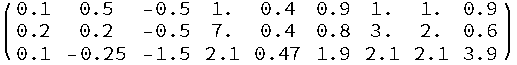
\includegraphics{refHmat.pdf}}}\intertext{with $\psi_c=\psi_\epsilon=0, \,\,  \psi_z=I$.
These coefficients are not completely arbitrary in so far as the series 
representation requires that the linear model
has a unique stable solution.}
  B=
\vcenter{\hbox{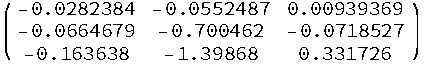
\includegraphics{refBmat.pdf}}}\\
\phi=
\vcenter{\hbox{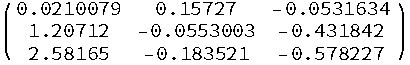
\includegraphics{refPhimat.pdf}}}\\
F=
\vcenter{\hbox{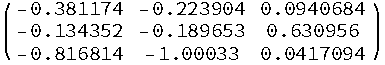
\includegraphics{refFmat.pdf}}}
\end{gather} 



The existence of a series 
representation requires only that the state values along the 
paths remain bounded.  For example, consider the following three
bounded families of time series paths:
\begin{gather}
  x_{1,t}=\alpha D_\pi(t) \\
x_{2,t}=\beta (-1)^t\\
x_{3,t}=\epsilon_t 
\end{gather} 
where $D_\pi(t)$ gives the t-th digit of $\pi$ and the $\epsilon_t$ are a sequence of pseudo random draws from the uniform distributions $\mathcal{U}(-4,4)$

In Figure \ref{arbpaths}, the first set of trajectories characterizes 
a function of the digits in the decimal representation of $\pi$.  
The second set of trajectories  oscillates between two values
determined by  a nonlinear function of the initial conditions and the shock.
The third set of trajectories characterizes a sequence of uniformly distributed random numbers based on a seed determined by  a nonlinear function of  the initial conditions and the shock.
These examples paths were chosen to emphasize that the trajectories
 need not converge to a fixed point, and 
need not be produced by iteration of a discrete-time map.
The boundedness of the paths is a sufficient condition for the existence 
of the series representation based on the ``almost arbitrary'' linear reference model,$\linMod$.\footnote{Although useful in some contexts,
this paper will not investigate representations for families of
unbounded trajectories.}


\begin{figure}
  \centering
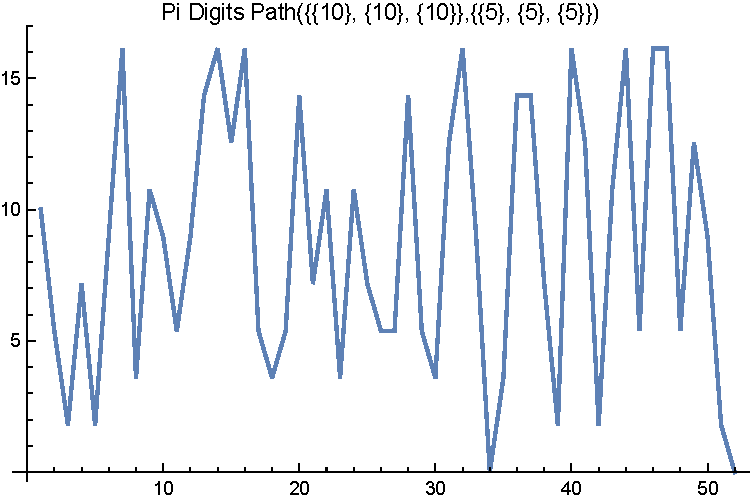
\includegraphics[width=2in]{piPath.pdf}
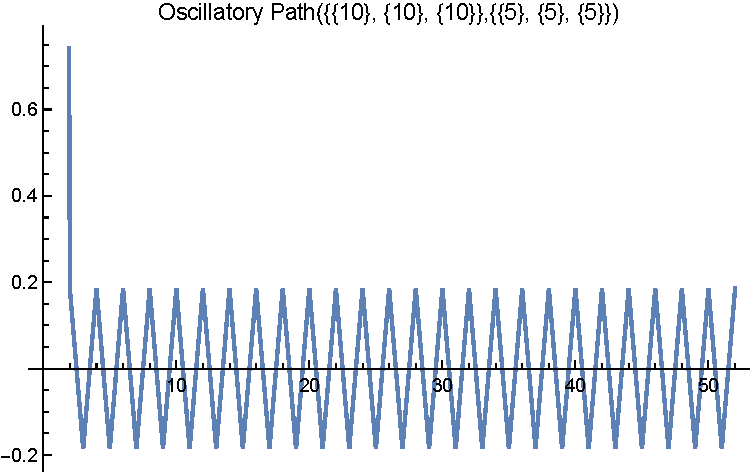
\includegraphics[width=2in]{oscillPath.pdf}
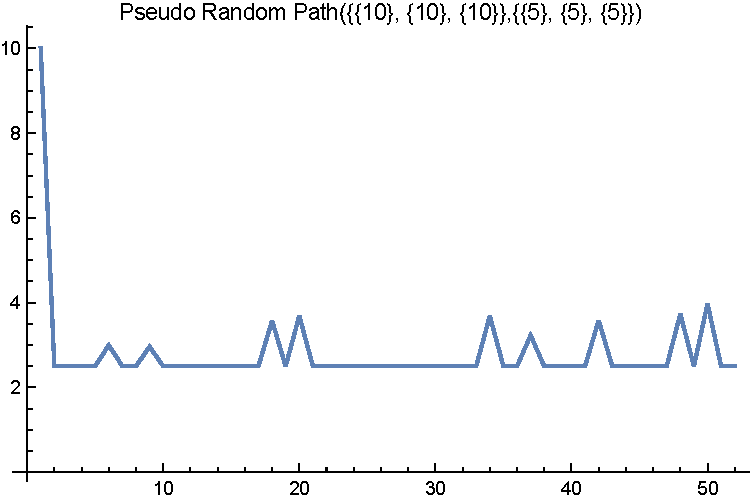
\includegraphics[width=2in]{pseudoPath.pdf}
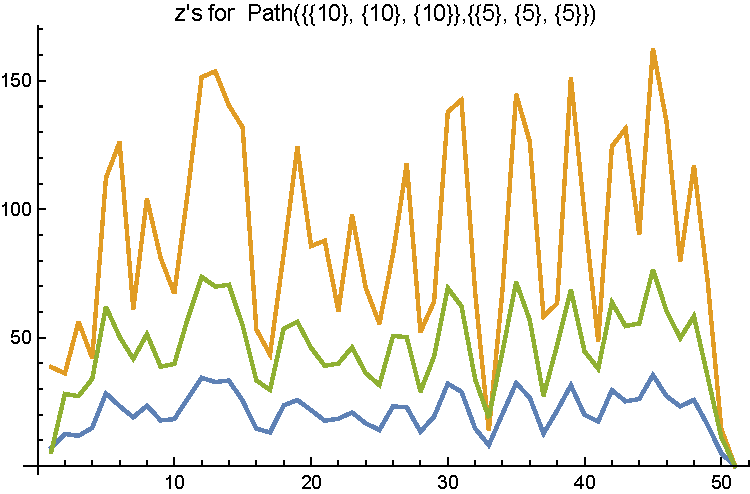
\includegraphics[width=3in]{theZs.pdf}  
  
  \caption{Arbitrary Bounded Time Series Paths and Corresponding $z_{i,t}$ values}\label{arbpaths}
\end{figure}





Figure \ref{arbpaths} also shows, for a particular initial state vector and shock value,  the paths for the state vectors and the  z's that generate the path.
One can repeat the calculations for any given initial condition to produce
a z series exactly replicating the given set of trajectories.  Thus, the family
of z functions along with equation \ref{theSeries} provide a series 
representation for the family of trajectories. 





\subsection{Assessing $x_t$ Errors}
\label{sec:truncationerr}
The formula \ref{theSeries} was derived to compute he impact on the current state of fully anticipated future shocks.  The formula characterizes the impact exactly.  However one can contemplate the impact of at least two types of imprecision.  One could truncate a series of correct values of $z_t$.  One might have imprecise values of $z_t$ along the path.

\subsubsection{Truncation Error}


One could consider approximating $\mathcal{X}_t$ by 
truncating the series \ref{theSeries} at a finite number of terms.
 	 \begin{gather}
 	 \xWOargK_t \equiv B x_{t-1}+ \phi \psi_\epsilon\epsilon  + (I - F)^{-1} \phi \psi_c + \sum_{s=0}^k F^s \phi z_{t}\label{theTruncSeries}
 \end{gather}
We can bound the  series approximation truncation errors.
Since
    \begin{gather}
      \label{eq:1}
\sum_{s=k+1}^{\infty} F^s \phi \psi_z = (I -F)^{-1} F^{k+1}\phi \psi_z       \\
\infNorm{\xWarg-\xWargK} \le \infNorm{(I -F)^{-1} F^{k+1}\phi \psi_z} \left ( \infNorm{H_{-1} }+ \infNorm{H_{0} }+ \infNorm{H_{1} } \right )\bar{\mathcal{X}}
    \end{gather}
Note that for approximating $\xWarg$ the impact of  a given realization along the path declines for those realizations which are  more temporally distant.

 Figure \ref{figArbTrunc} shows
that the truncation error bound is a very conservative measure of the accuracy
of the truncated series.  The orange line represents the computed bound of
the infinity norm of the difference between $x_t$ from the full series and a truncated series for different lengths of the truncation.  The blue line shows the infinity norm of the actual difference between the $x_t$ computed using the full series and the value obtained using a truncated series.  The series requires only the first 20 terms to compute
the initial value of the state vector to machine precision. 
The series representation can compute the entire series to machine precision
if all the terms are included, but the terms for state vectors closer 
to the initial time have the most important impact.


\begin{figure}
  \centering


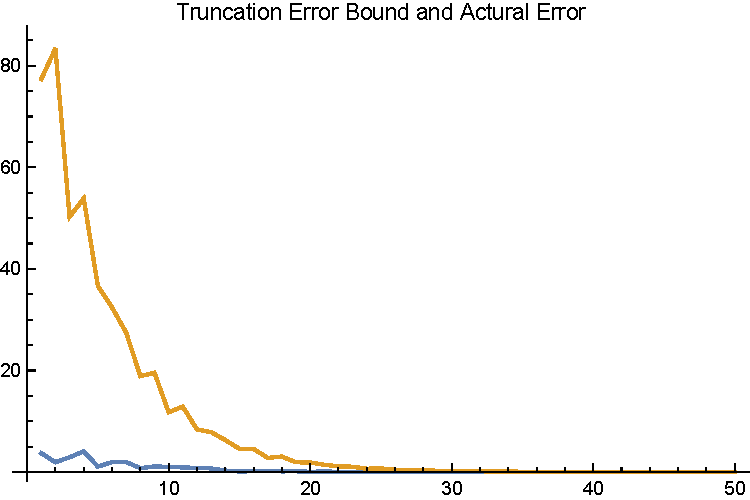
\includegraphics[width=3in]{arbTruncErr.pdf}  
  \caption{$x_t$ Error Bound Versus Actual Error} \label{figArbTrunc}

\end{figure}

\subsubsection{Path Error}


We can assess the impact of incorrect values for $z_t$ by computing the maximum correction required for the $z_t$ and applying the 
same formula.
One could consider approximating $\mathcal{X}_t$ using
 	 \begin{gather}
 	 \xWOargK_t \equiv B x_{t-1}+ \phi \psi_\epsilon\epsilon  + (I - F)^{-1} \phi \psi_c + \sum_{s=0}^\infty F^s \phi (z_{t}+\Delta z_{t})\label{theDeltaSeries}
 \end{gather}
Note that for approximating $\xWarg$ the impact of  a given realization along the path declines for those realizations which are  more temporally distant.
However, we can bound the  series approximation  errors by using the largest $\Delta z_t$ in the formula. 
Since
    \begin{gather}
\infNorm{\xWarg-\xWargK} \le \infNorm{(I -F)^{-1} \phi \psi_z}  \infNorm{\Delta z_t } \label{pathErr}
    \end{gather}


\label{sec:pathnorm}

\section{Nonlinear Dynamic Stochastic Time Invariant Maps}
\label{sec:extToMaps}



\subsection{Application to Time Invariant Maps}


In this paper we will be interested in computing with time
 invariant maps. Many dynamic stochastic models have solutions that 
fall in this class. 
These time invariant maps generate  bounded time series paths which can
be represented using the framework from section \ref{sec:newseries}.
These time invariant maps impose additional structure on the time 
series they generate.  This structure will allow us to use the series formula to
develop bounds for the error in the solution.
In this section, to keep things simple, we will rule out regime switching and occasionally binding constraints and start
 with  a simple single equation system?
Later, in order to handle models with regime switching and occasionally binding constraints, will need to consider more complicated collections of 
of equation systems with  Boolean gates. We will show how to apply the 
series formulation to get error bounds for these models as well.



\subsection{An RBC Example}
\label{sec:rbcaux}
  We consider a model described in \cite{Maliar2005}\footnote{Here, we set their $\beta=1$ do not discuss quasi-geometric discounting or time-inconsistency.}
 \begin{gather*}
   \max\left \{  u(c_t) + E_t \sum_{t=0}^\infty  \delta^{t}u(c_{t+1})\right \}\\
c_t + k_t=(1-d)k_t + \theta_t f(k_t)\\
f(k_t)= k_t^\alpha\\
u(c)=\frac{c^{1-\eta}-1}{1-\eta}
 \end{gather*}
The well known first order conditions for the model are

\begin{tcolorbox}[ams gather]
\frac{1}{c_t^{\eta}}=\alpha \delta k_{t}^{\alpha-1} E_t \left (\frac{\theta_{t+1}}{c_{t+1}^\eta} \right ) \\
c_t + k_t=\theta_{t-1}k_{t-1}^\alpha \\
 \theta_t =\theta_{t-1}^\rho e^{\epsilon_t}\label{rbcSys}
 \end{tcolorbox}



\label{sec:rbcexample}

When $\eta=d=1$, we have

 \begin{gather}
\frac{1}{c_t}=\alpha \delta k_{t}^{\alpha-1} E_t \left (\frac{\theta_{t}}{c_{t+1}} \right ) \\
c_t + k_t=\theta_{t-1}k_{t-1}^\alpha \\
\theta_t =\theta_{t-1}^\rho e^{\epsilon_t}\label{rbcSys}
\intertext{and there is a closed form solution}
c_t=  (1-\alpha \delta) \theta_{t} k_{t-1}^\alpha\\
  k_{t}= \alpha \delta \theta_{t} k_{t-1}^\alpha.\label{soln}\\
\theta_t =\theta_{t-1}^\rho e^{\epsilon_t}.
\end{gather}
For mean zero iid $\epsilon_t$ we can easily 
compute the conditional expectation of the model variables for any given $\theta_{t-1},k_{t-1}$
\begin{gather*}
  E_t(c_t|\theta_{t-1},k_{t-1})=(1-\alpha\delta)k_{t-1}^\alpha e^{\frac{\sigma^2}{2}}\theta_{t-1}^\rho\\
  E_t(k_t|\theta_{t-1},k_{t-1})=\alpha\delta k_{t-1}^\alpha e^{\frac{\sigma^2}{2}}\theta_{t-1}^\rho\\
  E_t(\theta_t|\theta_{t-1},k_{t-1})=e^{\frac{\sigma^2}{2}}\theta_{t-1}^\rho
\end{gather*}


By applying the law of iterated expectations, we can compute conditional expected solution paths forward from any initial values $x_{t-1}$
and realization of $\epsilon_t$.
As a result, we can use the family of conditional expectations
along with the contrived reference model to recover an 
approximation for equation \refeq{soln} along with error bounds.
The series representation provides a weighted sum of $z_t\tArg$ functions that give us
an approximation for the known solution.
Note that the reference model is deterministic and the $z_t\tArg$ functions account for the stochastic nature of the model.

For any given values of $k_{t-1},\theta_{t-1}, \epsilon_t$ the model solution and conditional expectations path produces paths for $z_{1t}\tArg, z_{2t}\tArg, z_{3t}\tArg$

\begin{gather*}
  \begin{bmatrix}
c_t(k_{t-1},\theta_{t-1}, \epsilon_t)\\
k_t(k_{t-1},\theta_{t-1}, \epsilon_t)\\
\theta_t(k_{t-1},\theta_{t-1}, \epsilon_t)
  \end{bmatrix} \rightarrow
  \begin{bmatrix}
  z_{1t}(k_{t-1},\theta_{t-1}, \epsilon_t)\\
  z_{2t}(k_{t-1},\theta_{t-1}, \epsilon_t)\\
  z_{3t}(k_{t-1},\theta_{t-1}, \epsilon_t) 
  \end{bmatrix}\equiv z(k_{t-1},\theta_{t-1}, \epsilon_t)\intertext{where}
  \begin{bmatrix}
c_t(k_{t-1},\theta_{t-1}, \epsilon_t)\\
k_t(k_{t-1},\theta_{t-1}, \epsilon_t)\\
\theta_t(k_{t-1},\theta_{t-1}, \epsilon_t)
  \end{bmatrix}  =
B   \begin{bmatrix}
c_{t-1}\\
k_{t-1}\\
\theta_{t-1}
  \end{bmatrix}  + \phi \psi_\epsilon\epsilon_t + (I - F)^{-1} \phi \psi_c + \sum_{\sForSum=0}^\infty F^s \phi z_{t+\sForSum}(k_{t-1},\theta_{t-1}, \epsilon_t) 
\end{gather*}
% \footnote{
% We need not  make these adjustments for the steady state,
% but doing so economizes on the number of terms 
% required for a given level of approximation
% accuracy.}

For example, using the following parameter values and using the arbitrary linear reference model we can generate a series representation for the model solutions.

\begin{gather}\label{rbcparams}
\vcenter{\hbox{\includegraphics{../../paperProduction/occBind/docs/RBCParamSubs.pdf}}} \,\, \text{ we have } \,\,
  \begin{bmatrix}
    c_{ss}\\k_{ss} \\ \theta_{ss} 
  \end{bmatrix}=
\left [ \vcenter{\hbox{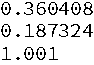
\includegraphics{RBCSSVal.pdf}}}\right ]
\end{gather}

With 
\begin{gather}\label{theInits}
  \begin{bmatrix}
 k_{t-1}\\\theta_{t-1}\\\epsilon_t 
  \end{bmatrix}=
\left [ \vcenter{\hbox{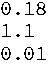
\includegraphics{anXEps.pdf}}}\right ]
\end{gather}


\begin{figure}
  \centering
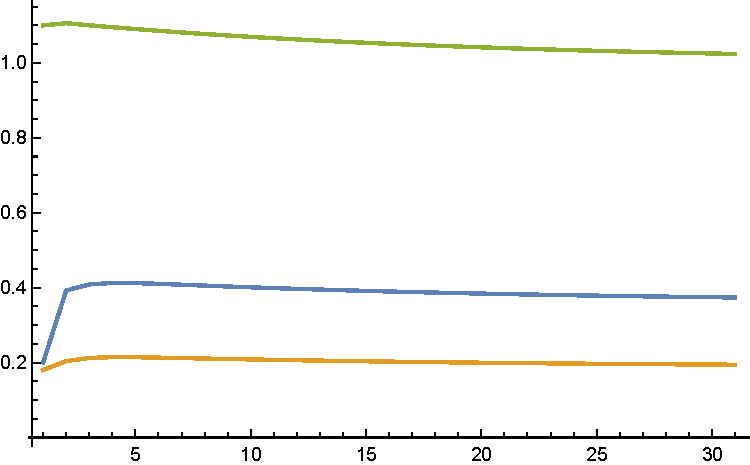
\includegraphics[width=2.5in]{simprbcvals.pdf}  
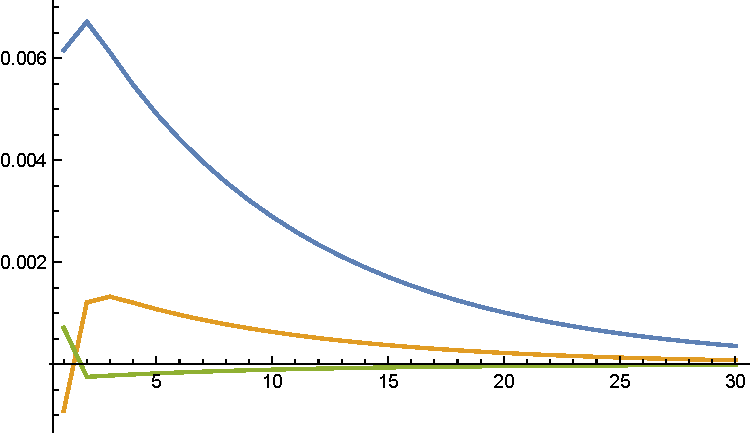
\includegraphics[width=2.5in]{simprbczvals.pdf}  
  \caption{model variable values and z values}
  \label{rbcpaths}
\end{figure}

The left panel of Figure \refeq{rbcpaths} shows the paths, from top to bottom, of $\theta_t, c_t, \text{and} k_t$ from the initial values given in Equation \refeq{theInits}.  The right panel shows the paths for the $z_t$ variables associated with the linear reference model. The orange line corresponds to $z_{1t}\tArg$,
the blue line corresponds to $z_{2t}\tArg$ and the green line corresponds to $z_{3t}\tArg$.

Figure \ref{rbcTrunc} shows the impact that truncating the series has 
on the initial value of the state variables.   The bound, $B_n$, shown in red 
again is very pessimistic compared to the actual, $Z_n$, shown in blue.
 But even with an arbitrarily chosen linear model, ultimately the series approximation provides an accurate value for the initial state vector.  

\begin{figure}
  \centering
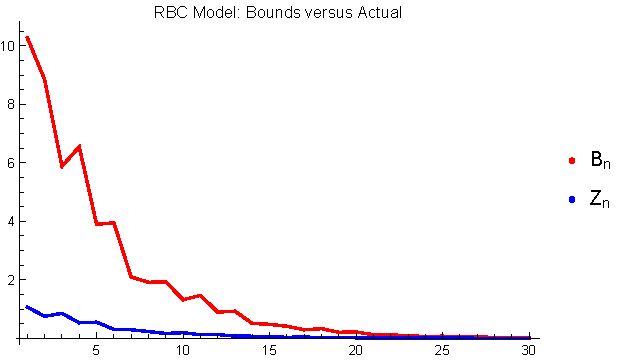
\includegraphics[width=2.7in]{simpArbBoundsVActual.pdf}  
  \caption{RBC Truncation Error Bound Versus Actual}
  \label{rbcTrunc}
\end{figure}
\begin{figure}
  \centering
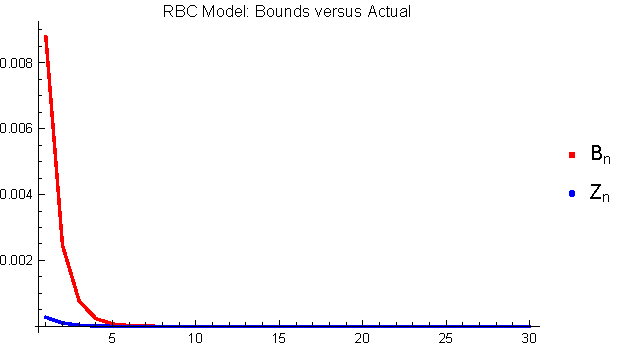
\includegraphics[width=2.7in]{simpBoundsVActual.pdf}  
  \caption{RBC Truncation Error Bound Versus Actual}
  \label{rbcTruncSimp}
\end{figure}



Figure \ref{rbcTruncSimp} shows that using a 
linearization that better tracks the 
nonlinear model paths, improves the approximation $Z_n$, shown in blue  and the error bound $B_n$ shown in red.
Using the linearization of the RBC model produces a tighter but still pessimistic bound on the errors for the initial state vector.
The first few terms make most of the difference in approximating the value of the state variables.




For convenience of notation in what follows, 
we will focus on models built up from components of the form
\begin{gather}
  h_i(x_{t-1},x_{t},x_{t+1},\epsilon_t)=h^{det}_{io}(x_{t-1},x_{t},\epsilon_t)+\sum_{j=1}^{p_i} [h^{det}_{ij}(x_{t-1},x_{t},\epsilon_t)h^{nondet}_{ij}(x_{t+1})]=0
\end{gather}
This is a very broad class of models including most widely used
macroeconomics models.

For example, the Euler equations for the  neoclassical growth  model 
\label{sec:simple-rbc-model-ext} can be written as
\begin{gather}
h_{10^{det}}(\cdot)=\frac{1}{c_t^\eta},\,\,
h_{11}^{det}()=\alpha \delta k_{t}^{\alpha-1} ,\,\,
h_{11}^{nondet}(\cdot)=E_t \left (\frac{\theta_{t+1}}{c_{t+1}^\eta} \right )\\
h_{20}^{det}(\cdot)=c_t + k_t-\theta_tk_{t-1}^\alpha,\,\,
h_{21}^{det}(\cdot)=0\\
h_{30}^{det}(\cdot)=\ln \theta_t -(\rho \ln \theta_{t-1} + \epsilon_t),\,\,
h_{31}^{det}(\cdot)=0
\end{gather}
Since we would otherwise  need to compute 
the conditional expectation of nonlinear expressions,  
this setup will make it possible for us to use auxiliary
variables to correctly compute the required expected values.

It is worth noting that since we will be working with models where expectations are computed at time t, with  $\epsilon_t$  known,  the only stochastic components are those with time subscripts greater than $t$. 





We now construct our linear reference model by increasing its dimension by one , $\linMod$, to accommodate 
 augmenting the RBC model with the equation
\begin{tcolorbox}[ams gather]
  \rcpC_t=\frac{\eta}{c_t}
\end{tcolorbox}
substituting $\rcpC_{t+1}$ for $\frac{1}{c_{t+1}}$ in the first equation and 
 linearizing the RBC model about the ergodic mean
given in \refeq{rbcparams}
{\small
\begin{gather}
  \begin{bmatrix}
H_{-1}&H_{0}&H_{1} 
  \end{bmatrix}=\\
\vcenter{\hbox{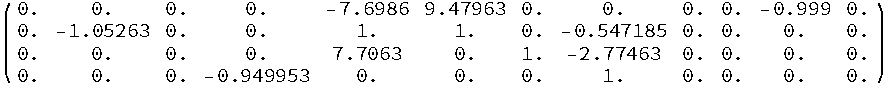
\includegraphics{RBCHmatSymb.pdf}}} \label{rbcLinSys}
\intertext{with}
\psi_\epsilon=
\begin{bmatrix}
  0\\0\\1\\0
\end{bmatrix}, \psi_z=I
\end{gather}%(\footnote{generated by AMAPaperCalcs.mth {RBCHmatSymb.pdf}})
}
These coefficients  produce a unique stable linear solution.

\begin{gather}
  B=
\vcenter{\hbox{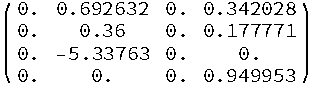
\includegraphics{RBCBmatSymb.pdf}}},
\phi=
\vcenter{\hbox{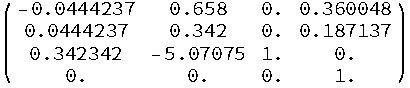
\includegraphics{RBCPhimatSymb.pdf}}}\\
F=
\vcenter{\hbox{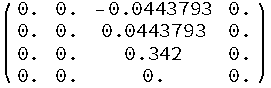
\includegraphics{RBCFmatSymb.pdf}}}\\
\psi_c=\vcenter{\hbox{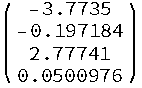
\includegraphics{RBCPsissSymb.pdf}}}
\end{gather}
\section{Computing Model Solution Error Bounds}
\label{sec:solnerrorbounds}


\subsection{Model Specification}
\label{sec:model-specification}


We will consider time invariant maps that arise form solving a time t optimization problem codified in a collection of systems of equations.  We will assume that we have a countable collection of equations systems that are mutually exclusive and exhaustive.  Given $\epsilon_t, x_{t-1}$,  this collection of 
systems of equations produces a unique solution for $x_t$.  We will include 
enough auxiliary variables so that we can correctly compute expected values
for model variables by applying the law of iterated 
expectations to individual variables.
The $x_t$ satisfies one and only one of the 
collection of equations and $x_t$ is (locally) the unique solution 
for the collection of
equations.  Examples of such systems include typical DSGE models that have one
system of equations, occasionally binding constraints with solutions demonstrating complementary slackness, regime switching models with systems corresponding to the status in each given regime or combinations of the above.

It will be convenient for describing the algorithms to
 augment the model equations to include auxiliary variables so that we can write the model in the form

\begin{gather}
\eqnFuncSys \intertext{ where, each }
\eqnFuncSysI{i}\equiv \eqnFuncSysIExpl{i} \label{eqnGates}
\end{gather}
 represents a set of model equations, $\eqnFunc_i$,  with a Boolean valued gate, $\gate_i$. Consequently, will will have an equation system and a gatekeeper logical expression indicating which equation system is in force for a given solution for a give $x_{t-1}, \epsilon_t$  They represent exhaustive and mutually exclusive equation systems determining the solution at time t for the model.  They could be complementary slackness conditions or could represent a model with different regimes. We will consider time invariant model solutions $x_t=\xWarg$.  Given $\xWarg$, $\XWOarg(x_{t-1})\equiv \expct{\xWarg}$. 




\subsubsection{Occasionally Binding Constraints}
\label{sec:obc-solut}



Consider adding constraints the constraints:

\begin{gather*}
  I_t \ge \upsilon I_{ss}
\end{gather*}


\begin{tcolorbox}[ams gather]
if(\mu>0 \land (k_t - (1-d)k_{t-1}-\upsilon I_{ss})=0)\\
  \lambda_t -\frac{1}{c_t}\\
c_t+I_t-\theta_tk_{t-1}^\alpha\\
N_t-\lambda_t \theta_t\\
\theta_t-e^{(\rho\ln(\theta_{t-1})+\epsilon)}\\
\lambda_t + \mu_t - (\alpha k_t^{(\alpha-1)}\delta N_{t+1}+\lambda_{t+1} \delta (1-d)+\mu_{t+1}+\delta (1-d)\mu_{t+1}\\
I_t-(K_t-(1-d)k_{t-1})\\
\mu_t(k_t - (1-d) k_{t-1}-\upsilon I_{ss})\\
\end{tcolorbox}
\begin{tcolorbox}[ams gather]
if(\mu=0 \land (k_t - (1-d)k_{t-1}-\upsilon I_{ss})\ge 0)\\
  \lambda_t -\frac{1}{c_t}\\
c_t+I_t-\theta_tk_{t-1}^\alpha\\
N_t-\lambda_t \theta_t\\
\theta_t-e^{(\rho\ln(\theta_{t-1})+\epsilon)}\\
\lambda_t + {\mu_t} - (\alpha k_t^{(\alpha-1)}\delta N_{t+1}+\lambda_{t+1} \delta (1-d)+{\mu_{t+1}}+\delta (1-d)\mu_{t+1}\\
I_t-(K_t-(1-d)k_{t-1})\\
\mu_t(k_t - (1-d) k_{t-1}-\upsilon I_{ss})
\end{tcolorbox}


\subsubsection{Regime Switching}


\label{sec:regime-switch-model}

\begin{itemize}
\item best to have a functional form for each regime.
\item conditional expectation probability transition just weighted sums
\item to make transition probability a function of state 
can(should>) use same grid for $p_{ij}(x)$  will get a different conditional expectations polynomial at each x
\item can use for heterogeneous agents
\end{itemize}


Consider two states $s_t \in {0,1}$ where the depreciation rates are different:  $d_0>d_1$

\begin{gather}
    Prob(s_t=j|s_{t-1}=i)=p_{ij}
\end{gather}

For example, the Euler equations for the  neoclassical growth  model 
\label{sec:simple-rbc-model-ext} can be written as
\begin{tcolorbox}[ams gather]
if(s_t=0\land \mu>0 \land (k_t - (1-d_0)k_{t-1}-\upsilon I_{ss})=0)\\
  \lambda_t -\frac{1}{c_t}\\
c_t+k_t-\theta_tk_{t-1}^\alpha\\
N_t-\lambda_t \theta_t\\
\theta_t-e^{(\rho\ln(\theta_{t-1})+\epsilon)}\\
\lambda_t + {\mu_t} - (\alpha k_t^{(\alpha-1)}\delta N_{t+1}+\lambda_{t+1} \delta (1-d_0)+{\mu_{t+1}}+\delta (1-d_0)\\
I_t-(K_t-(1-d_0)k_{t-1})\\
\mu_t(k_t - (1-d_0) k_{t-1}-\upsilon I_{ss})\\
\end{tcolorbox}
\begin{tcolorbox}[ams gather]
if(s_t=0\land\mu=0 \land (k_t - (1-d_0)k_{t-1}-\upsilon I_{ss})\ge 0)\\
  \lambda_t -\frac{1}{c_t}\\
c_t+k_t-\theta_tk_{t-1}^\alpha\\
N_t-\lambda_t \theta_t\\
\theta_t-e^{(\rho\ln(\theta_{t-1})+\epsilon)}\\
\lambda_t + {\mu_t} - (\alpha k_t^{(\alpha-1)}\delta N_{t+1}+\lambda_{t+1} \delta (1-d_0)+{\mu_{t+1}}+\delta (1-d_0)\\
I_t-(K_t-(1-d_0)k_{t-1})\\
\mu_t(k_t - (1-d_0) k_{t-1}-\upsilon I_{ss})
\end{tcolorbox}
\begin{tcolorbox}[ams gather]
if(s_t=1\land \mu>0 \land (k_t - (1-d_1)k_{t-1}-\upsilon I_{ss})=0)\\
  \lambda_t -\frac{1}{c_t}\\
c_t+k_t-\theta_tk_{t-1}^\alpha\\
N_t-\lambda_t \theta_t\\
\theta_t-e^{(\rho\ln(\theta_{t-1})+\epsilon)}\\
\lambda_t + {\mu_t} - (\alpha k_t^{(\alpha-1)}\delta N_{t+1}+\lambda_{t+1} \delta (1-d_1)+{\mu_{t+1}}+\delta (1-d_1)\\
I_t-(K_t-(1-d_1)k_{t-1})\\
\mu_t(k_t - (1-d_1) k_{t-1}-\upsilon I_{ss})\\
\end{tcolorbox}
\begin{tcolorbox}[ams gather]
if(s_t=1\land\mu=0 \land (k_t - (1-d_1)k_{t-1}-\upsilon I_{ss})\ge 0)\\
  \lambda_t -\frac{1}{c_t}\\
c_t+k_t-\theta_tk_{t-1}^\alpha\\
N_t-\lambda_t \theta_t\\
\theta_t-e^{(\rho\ln(\theta_{t-1})+\epsilon)}\\
\lambda_t + {\mu_t} - (\alpha k_t^{(\alpha-1)}\delta N_{t+1}+\lambda_{t+1} \delta (1-d_1)+{\mu_{t+1}}+\delta (1-d_1)\\
I_t-(K_t-(1-d_1)k_{t-1})\\
\mu_t(k_t - (1-d_1) k_{t-1}-\upsilon I_{ss})
\end{tcolorbox}

\subsection{The Formula}
\label{sec:errorformula}


In what follows, we construct an error bound for proposed model solutions.



 Given an exact solution $x^\star_t=g^\star(x_{t-1},\epsilon_t)$ define
  \begin{gather}
G^\star(x)\equiv\expct{g^\star(x,\epsilon)} \intertext{then with}
E_tx^\star_{t+1}=G^\star(g^\star(x_{t-1},\epsilon_t))\\
    \label{eq:2}
\eqnFunc(x^\star_{t-1},x^\star_t,E_tx^\star_{t+1},\epsilon_t)=0  \,\, \forall  (x_{t-1},\epsilon_t)\\ \intertext{Using $G^\star$ and $\linMod$ construct the family of trajectories and corresponding $z^\star_t(x_{t-1},\epsilon)$ }
   x^\star_t(x_{t-1},\epsilon_t) \in{R^L}\,\,\infNorm{x^\star_t(x_{t-1},\epsilon_t)}  \le \bar{\mathcal{X}}\,\,\forall t\ > 0
  \end{gather}
   \begin{align}
   z^\star_{t}(x_{t-1},\epsilon_t) \equiv& H_{-1}  x^\star_{t-1}(x_{t-1},\epsilon_t) + \nonumber\\
 & H_0  x^\star_{t}(x_{t-1},\epsilon_t) +  \label{defZ} \\
 & H_1  x^\star_{t+1}(x_{t-1},\epsilon_t). \nonumber
   \end{align}




   The exact solution has a representation given by
	 \begin{gather}
	 x^\star_{t}(x_{t-1},\epsilon) =B x_{t-1}+ \phi \psi_\epsilon\epsilon + (I - F)^{-1} \phi \psi_c +\\ \sum_{\sForSum=0}^\infty F^s \phi z^\star_{t+\sForSum}(x_{t-1},\epsilon) \intertext{and}
	 \expct{x^\star_{t+1}(x_{t-1},\epsilon)} =B x^\star_{t+k} + \sum_{\sForSum =0}^\infty F^\sForSum \phi \expct{z^\star_{t+1+\sForSum}(x_{t-1},\epsilon)} + (I - F)^{-1} \phi \psi_c 
 \intertext{with}
 \eqnFunc(x_{t-1},x^\star_t,E_tx^\star_{t+1},\epsilon_t)=0  \,\, \forall  (x_{t-1},\epsilon_t)\\ 
	 \end{gather}

Now consider a proposed solution for the model,
 $x^p_t=g^p(x_{t-1},\epsilon_t)$ define
$G^p(x)\equiv\expct{g^p(x,\epsilon)}$  so that 
  \begin{gather}
E_tx_{t+1}=G^p(g^p(x_{t-1},\epsilon_t))\\
\mathbf{e}_t(x_{t-1},\epsilon)\equiv
\eqnFunc(x_{t-1},x^p_t,E_tx^p_{t+1},\epsilon_t)\\\intertext{Using $G^p$ and $\linMod$ construct the family of trajectories and corresponding $z^p_t(x_{t-1},\epsilon)$ }
   x^p_t(x_{t-1},\epsilon_t) \in{R^L}\,\,\infNorm{x^p_t(x_{t-1},\epsilon_t)}  \le \bar{\mathcal{X}}\,\,\forall t\ > 0
  \end{gather}
   \begin{align}
   z^p_{t}(x_{t-1},\epsilon_t) \equiv& H_{-1}  x^p_{t-1}(x_{t-1},\epsilon_t) + \nonumber\\
 & H_0  x^p_{t}(x_{t-1},\epsilon_t) +  \label{defZ} \\
 & H_1  x^p_{t+1}(x_{t-1},\epsilon_t). \nonumber
   \end{align}








 The proposed solution has a representation given by 
  \begin{gather}
    \label{eq:4}
	 x^p_{t}(x_{t-1},\epsilon) =B x_{t-1}+ \phi \psi_\epsilon\epsilon + (I - F)^{-1} \phi \psi_c +\\ \sum_{\sForSum=0}^\infty F^s \phi z^p_{t+\sForSum}(x_{t-1},\epsilon) 
 \intertext{and}
 	 \expct{x^p_{t+1}(x_{t-1},\epsilon)} =B x^p_{t+k} + \sum_{\sForSum =0}^\infty F^\sForSum \phi z^p_{t+1+\sForSum}(x_{t-1},\epsilon) + (I - F)^{-1} \phi \psi_c \intertext{with}
\mathbf{e}_t(x_{t-1},\epsilon)\equiv
\eqnFunc(x_{t-1},x^p_t,E_tx^p_{t+1},\epsilon_t)
  \end{gather}




  \begin{gather}
    \label{eq:3}
	 x^\star_{t}(x_{t-1},\epsilon) -	 x^p_{t}(x_{t-1},\epsilon) =
\sum_{\sForSum=0}^\infty F^s \phi (z^\star_{t+\sForSum}(x_{t-1},\epsilon)-z^p_{t+\sForSum}(x_{t-1},\epsilon))     \\
	 x^\star_{t}(x_{t-1},\epsilon) -	 x^p_{t}(x_{t-1},\epsilon) =
\sum_{\sForSum=0}^\infty F^s \phi \Delta z_{t+\sForSum}(x_{t-1},\epsilon_t)   \\ 
	\infNorm{ x^\star_{t}(x_{t-1},\epsilon) -	 x^p_{t}(x_{t-1},\epsilon)} \le
\sum_{\sForSum=0}^\infty F^s \phi \infNorm{\Delta z_{t+\sForSum}(x_{t-1},\epsilon_t)}    
  \end{gather}

By bounding the largest deviation in the paths for the $\Delta z_t$ we can bound the largest different in $x_t$.  The exact solution satisfies the model equations exactly.  The error in the proposed solution provides a conservative bound on the largest change in $z$.


  \begin{gather}
  \Delta z_t \le  \label{eq:3}
\max_{\{x_{-},\epsilon\}} \infNorm{ \phi \eqnFunc(x_{-},g^p(x_{-},\epsilon),G^p(g^p(x_{-},\epsilon)),\epsilon) }\\
	\infNorm{ x^\star_{t}(x_{t-1},\epsilon) -	 x^p_{t}(x_{t-1},\epsilon)} \le
\max_{\{x_{-},\epsilon\}} \infNorm{(I-F)^{-1} \phi \eqnFunc(x_{-},g^p(x_{-},\epsilon),G^p(g^p(x_{-},\epsilon)),\epsilon) }
  \end{gather}






\subsection{Practical Considerations for Applying the Formula}
\label{sec:practicalformula}



 
This section describes a method for finding maxima in a closed bounded domain.
Let $D=[a,b]$ in $R^s$ where $a_i \le x_i \le b_i$. We want to find  $M=f(x^\ast)= \max_{x \in D}f(x)$.
Th number theoretic (Quasi-Monte Carlo) approached is designed for finding optima with many local optima.  It is based on the used of space filling points.\cite{Xu2005}
The number theoretic method of optimization includes two basic steps.
\begin{enumerate}
\item Choose a set $p=x_i, i=1,\dots,n$ of potential optima that are uniformly scattered.
\item Find $M_n\text{ and } x^\ast \in p =\max_{1\le i \le n}f(x_i)$
\end{enumerate}

Even when choosing $p$ wisely convergence slow until \cite{Niederreiter1983}.  They speed up the convergence by contracting the domain.
Their algorithm discards all but the best in the domain. Must have very many points to guarantee choosing a point close to the optimum.


MSNTO selects a finite number of sample points uniformly scattered on D.  Next it discard inferior points retaining small sample of potential maxima.  These form the clusters for the next step.  The algorithm performs a domain contraction on each of the clusters.






\section{Improving Proposed  Solutions}
\label{sec:algoforsoln}

\begin{itemize}
\item It's a good idea to compute easy approximation using just the linear model one ieration to get an approximation for the ergodic set
\item them simulate and make the Maliar SVD transformation
\item then iterate on the ergodic set till it settles down
\item in this way can avoid solutions which are explosive when iterated 
\item need to see if this works when honoring complimentary slackness
\end{itemize}


\subsection{Algorithm Overview}
\label{sec:pseudocode}
{
  \begin{itemize}
  \item Consider the single model case $  \eqnFunc(x_{t-1},x_t,\expct{x_{t+1}},\epsilon)=0$.  
\item We seek $\eqnFunc(x_{t-1},\xWOarg^\star\tArg,\XWOarg^\star(\xWOarg^\star\tArg),\epsilon)=0\,\,\forall \tArg $
\item Given a proposed model solution $x_t=\xWOarg^p\tArg$ compute $\XWOarg^p(x_{t-1})\equiv \expct{\xWOarg^p\tArg}$. 
\item we will use a linear reference model $\linMod  \equiv \linModMats$ 
to construct a series of $\zpWOarg$ functions that improve the accuracy of the proposed solution.
\end{itemize}
}



\begin{gather*}
 \intertext{We can define functions $\zpWOarg,\ZpWOarg$ by}
\zpWarg\equiv H
\begin{bmatrix}
x_{t-1}\\ \xpWarg\\ \XpWOarg(\xWarg)
\end{bmatrix}+\phi_\epsilon \epsilon_t+\phi_c\\
\ZpWOarg(x_{t-1})\equiv \expct{\zpWarg}
\end{gather*}
 \begin{itemize}
\item  define conditional expectations paths for $x_t, z_t$ -- {\color{green}Algorithm loop begins here.}
 \begin{gather*}
 x_{t+k+1}=\XWOarg(x_{t+k}),\,\,\,z_{t+k+1}=\ZWOarg(x_{t+k})\,\,\,\,  \forall k\ge 0      \end{gather*}
% \item
% it will be useful to construct an augmented decision rule,
% $\ADR\tArg\equiv
%   \begin{bmatrix}
%     x^p\tArg\\z^p\tArg
%   \end{bmatrix}$, initially $z^p\tArg=0$
   \end{itemize}

{Using the $\zpWarg$ Series}
{\small
  \begin{itemize}
  \item We get expressions for $x_t, \expct x_{t+1}$ consistent with $\linMod$ and the conditional expectations path
   \begin{gather*}
     \mathcal{X}_{t} =B x_{t-1}+ \phi \psi_\epsilon\epsilon + (I - F)^{-1} \phi \psi_c + \sum_{\sForSum=0}^\infty F^s \phi \ZWOarg(x_{t+\nu})\\
	\expct{ \mathcal{X}_{t+1}} =B \mathcal{X}_{t}  + (I - F)^{-1} \phi \psi_c+ \sum_{\sForSum =0}^\infty F^{\sForSum-1} \phi \ZWOarg(x_{t+\nu}) \,\,\,\,\,\forall t,k \ge  0
\end{gather*}
\item Use the model equations, $\eqnFuncSys$ and $x_t\tArg=\mathcal{X}_t\tArg$ to determine $\xppWarg, \zppWarg$
\item $\xpWarg=\xppWarg, \zpWarg=\zppWarg$ -- {\color{green}Repeat loop.}
  \end{itemize}
}


\subsection{{Some Algorithmic Details}}


  


\begin{enumerate}
\item Not required, but one can use a linearized version of some $\eqnFunc_i$  as the  linear reference model, $\linMod$.
\item Current implementation builds on the approach described in \cite{Judd2014}
  \begin{itemize}
  \item Approximate the ``boundaries'' for the ergodic set
  \item Decide upon the  degrees of approximation for the an-isotropic Smolyak polynomial representation
  \item Precalculate all integrals
  \end{itemize}
\item Uses the $\linMod$ linear decision rule as an initial guess for decision rule $\xpWarg$ to obtain conditional expectations function
\item Linearities in series expressions exploited
\item Highly parallelizable 
\end{enumerate}








\subsection{Algorithm Pseudo-code}
\label{sec:pseudocode}

\begin{enumerate}
\item Specify a (collection of) model equations systems(s) 
as in \refeq{eqnGates}.
For all relevant values of $\tArg$ there is one and only one solution $x_t\tArg$
\item specify a linear reference model
\item specify an initial guess for decision rule $\xWargK$ obtain conditional expectations function
\item decide upon the ranges for variables and the degrees of approximation for the an-isotropic Smolyak polynomial representation
\item decide upon $K$, the number of conditional expectations function recursive iterations.  Fewer means more truncation error. In effect, 
the algorithm imposes nonlinear constraints the for number of period specified 
and uses the linear reference model thereafter(ie $z_t+N=0, \forall N>K$
\item algorithm uses conditional expectation and model equations to produce an improved approximation to the decision rule.
\item the algorithm finds a solution to the system that constrains $x_t= x_g$ determining $x_t,z_t$ at the interpolation points for $x_{t-1},\epsilon_t$  This can be done in parallel
\item the data from the interpolation points is used to produce an updated decision rule
\end{enumerate}



It will be convenient for describing the algorithms to
 augment the model equations to include auxiliary variables so that we can write the model in the form
$  \eqnFunc(x_{t-1},x_t,\expct{x_{t+1}},\epsilon)=0$.  We will consider time invariant model solutions $x_t=\xWarg$.  Compute $\XWOarg(x_{t-1})\equiv \expct{\xWarg}$. We will have

\begin{gather}
\eqnFunc(x_{t-1},\xWarg,\XWOarg(\xWarg),\epsilon)=0 \intertext{Given a linear reference model,}
\linMod  \equiv \linModMats \intertext{we can define functions $\zWOarg$ by}
\zWarg\equiv H
\begin{bmatrix}
x_{t-1}\\ \xWarg\\ \XWOarg(\xWarg)
\end{bmatrix}+\phi_\epsilon \epsilon_t+\phi_c\intertext{compute $\ZWOarg$ }
\ZWOarg(x_{t-1})\equiv \expct{\zWarg}\intertext{define conditional expectations paths for $x_t, z_t$}
x_{t+k+1}=\XWOarg(x_{t+k}),\,\,\,z_{t+k+1}=\ZWOarg(x_{t+k})\,\,\,\,  \forall k\ge 0\\
	 \mathcal{X}_{t} =B x_{t-1}+ \phi \psi_\epsilon\epsilon + (I - F)^{-1} \phi \psi_c + \sum_{\sForSum=0}^\infty F^s \phi z_{t+\sForSum} 
\intertext{and}
	 \mathcal{X}_{t+1} =B \mathcal{X}_{t}  + (I - F)^{-1} \phi \psi_c+ \sum_{\sForSum =0}^\infty F^\sForSum \phi z_{t+\sForSum+1} \,\,\,\,\,\forall t,k \ge  0 \\
	\expct{ \mathcal{X}_{t+1}} =B \mathcal{X}_{t}  + (I - F)^{-1} \phi \psi_c+ \sum_{\sForSum =0}^\infty F^\sForSum \phi \expct{z_{t+\sForSum+1}} \,\,\,\,\,\forall t,k \ge  0\\
	\expct{ \mathcal{X}_{t+1}} =B \mathcal{X}_{t}  + (I - F)^{-1} \phi \psi_c+ \sum_{\sForSum =0}^\infty F^\sForSum \phi \ZWOarg(x_{t+\nu}) \,\,\,\,\,\forall t,k \ge  0
\end{gather}





The $g$ function uses equation \ref{theSeries} to construct values needed to evaluate the model equations.
\begin{gather}
  g(x_{t-1},\epsilon_t,z_t)=
  \begin{bmatrix}
    x_{t-1}\\
B x_{t-1}+ \phi \psi_\epsilon\epsilon + (I - F)^{-1} \phi \psi_c + \sum_{\sForSum=0}^K F^s \phi z_{t+\sForSum} \\
B x_{t}+   (I - F)^{-1} \phi \psi_c + \sum_{\sForSum=0}^K F^s \phi z_{t+\sForSum} \\
\epsilon_t
  \end{bmatrix}
\end{gather}
\begin{algorithm}
 \SetKwInOut{Input}{input}
 \SetKwInOut{Output}{output}
\Input{$\linMod$, $\sum_{\nu=1}^N F^{\nu-1} \phi z_{t+\nu}$}
$x_t(x_{t-1},\epsilon_t,z_t)=B x_{t-1} + (I-F)^{-1} \phi. \psi_c+\phi \psi_\epsilon \epsilon_t + \phi . \psi_z z_t + F\sum_{\nu=1}^N F^{\nu-1} \phi z_{t+\nu} $\;
$\expct{x_{t+1}}(x_{t-1},\epsilon_t,z_t)=B x_{t}(x_{t-1},\epsilon_t,z_t) + (I-F)^{-1} \phi. \psi_c + \sum_{\nu=1}^N F^{\nu-1} \phi z_{t+\nu} $\;
$g(x_{t-1},\epsilon_t,z_t)\equiv
\begin{bmatrix}
  x_{t-1}\\x_t(x_{t-1},\epsilon_t,z_t)\\\expct{x_{t+1}}(x_{t-1},\epsilon_t,z_t)\\ \epsilon_t
\end{bmatrix}
$\;
\Output{$g(x_{t-1},\epsilon_t,z_t)$}
\caption{$\modArgs(\linMod,\sum_{\nu=1}^N F^{\nu-1} \phi z_{t+\nu})$}
\label{gEqn}
\end{algorithm}

We will represent model solutions using the an-isotropic Smolyak interpolation method outlined in \cite{Judd2014}.\footnote{ This choice makes it possible to precompute all the integrals necessary for the conditional expectations calculations. See section \ref{sec:smolyakinterp} for details.}  This will require solving
the following system at a prespecified number of points.  This can be done in parallel. We can use the linear system associated with some 
linear reference model, $\linMod$, as the initial guess.  
It is not necessary, but it may be useful to use some linearization of the model, $\eqnFunc$.  Typically one would start with the initial values for $z_t\tArg=0$.

From the  trial value for the model solution codified in the $\ADR$, $\xWOarg^k\tArg$, we obtain the corresponding $\ADRCE$, $\XWOarg^k\tNo$ and, as
 shown in algorithm \ref{fSum}, using
a guess for $x_t\tArg$ we compute a conditional expectations path of length N from $\tArg$ forward.  We use the $\ADRCE$\ expressions for $Z^k$ to compute the expected values for future $z_t$. As shown in algorithm \ref{gEqn}, we 
will use these values in the formula \ref{theSeries} to compute $x_t$ and $\expct{x_{t+1}}$. Algorithm \ref{gEqn} provides all the arguments needed for solving the equation system, $\eqnFunc$.  Algorithm \ref{theSys} obtains  $\xWOarg^k\tArg,\zWOarg^k\tArg$ at the designated points so that the model equations are satisfied and the $\xguss=x$

\begin{algorithm}
 \SetKwInOut{Input}{input}
 \SetKwInOut{Output}{output}
\Input{$\linMod$, $\xguss$, $\XWOarg^k$, $\ZWOarg^k$, $N$}
$x_{t+1}=\XWOarg^k(\xguss)$\;
$z_{t+1}=\ZWOarg^k(\xguss)$\;
\For{$i=2$ to $N$}{
$x_{t+i}=\XWOarg^k(x_{t+i-1})$\;
$z_{t+i}=\ZWOarg^k(x_{t+i-1})$\;
}
\Output{$\sum_{\nu=1}^N F^{\nu-1} \phi z_{t+\nu}$}
\caption{$\fSum(\linMod, \xguss, \XWOarg^k, \ZWOarg^k, N)$} 
\label{fSum}
\end{algorithm}


\begin{algorithm}
 \SetKwInOut{Input}{input}
 \SetKwInOut{Output}{output}
\Input{$\eqnFunc$, $\linMod$,  $\XWOarg^k$, $\ZWOarg^k$, $N$, $x_{t-1}$, $\epsilon_t$}
Find $x_t$ and $z_t$
$\eqnFunc(\modArgs(\linMod,\fSum(\linMod,\xguss,\XWOarg^k,\ZWOarg^k)))=0$\;
$\xguss=x_t(x_{t-1},\epsilon)$\;
\Output{$\xWOarg^{k+1}(x_{t-1},\epsilon_t)$, $\zWOarg^{k+1}(x_{t-1},\epsilon_t)$}
\caption{$\xWOarg^{k+1}(x_{t-1},\epsilon_t)$, $\zWOarg^{k+1}(x_{t-1},\epsilon_t)$}
\label{theSys}
\end{algorithm}


\subsection{Function Approximation Representation}
\label{sec:funcApproxRep}

\subsubsection{General Issues}
\label{sec:generalissues}










\subsubsection{Smolyak Interpolation}
\label{sec:smolyakinterp}

\paragraph{An-isotropic}
It is possible to precompute each of the integrals. Since the solution will be linear combination of the polynomials, precomputing the polynomials means the weighted sum of the precomputed integrals will provide the integrals.
\paragraph{Precomputing Integrals}
\begin{algorithm}
  \SetKwInOut{Input}{input}
 \SetKwInOut{Output}{output}
\Input{$\aSmolPoly$, $\smolRngs$, $\distribSpec$} 
\Output{$\int \aSmolPoly \Pi (f_i(\epsilon_i)) d\epsilon_1 \ldots d\epsilon_k$}
\end{algorithm}





\subsection{RBC Example}
\label{sec:rbc-example}


\subsubsection{Approximating the Known Solution: $U(c) = Log(c)$ }
\label{sec:recov-known-solut}

\begin{itemize}
\item for linear init iters =1 varying bigK has no effect
\item for linear init iters =2 varying bigK has some effect
\item msnto predicted and actual err added to graphs
\item 3D to 2D since epsilon doesn't matter much
\item big change from linear to nonliner iter >1
\item should use tErrMat * checkPt for ``closer error bound''
\item need \LaTeX conditional for mac runs instead of linux
\begin{verbatim}
In[14]:= !grep -l chooseLower resDir/*
resDir/forBetterRBC${1,1,4}Iters10theK1numKern0.mth
resDir/forBetterRBC${1,1,4}Iters10theK1numKern48.mth
resDir/forBetterRBC${1,1,4}Iters10theK5numKern48.mth
resDir/forBetterRBC${1,1,4}Iters20theK1numKern48.mth
resDir/forBetterRBC${1,1,4}Iters20theK20numKern48.mth
resDir/forBetterRBC${1,1,5}Iters10theK1numKern48.mth
resDir/forBetterRBC${1,1,5}Iters1theK10numKern48.mth
resDir/forBetterRBC${1,1,5}Iters1theK1numKern48.mth
resDir/forBetterRBC${1,1,5}Iters1theK20numKern48.mth
resDir/forBetterRBC${1,1,5}Iters1theK5numKern48.mth
resDir/forBetterRBC${1,1,5}Iters20theK10numKern48.mth

\end{verbatim}
\end{itemize}
Figure \ref{fig:erg}  characterizes the use of the parallelotope
transformation described in \cite{Judd2013}. The left panel shows the 200 values of $k_t$ and $\theta_t$ resulting from a stochastic simulation of the the known decision rule. The right panel shows the transformed variables the constitute
an improved set of variables for constructing function approximation values.
\begin{figure}
  \centering
  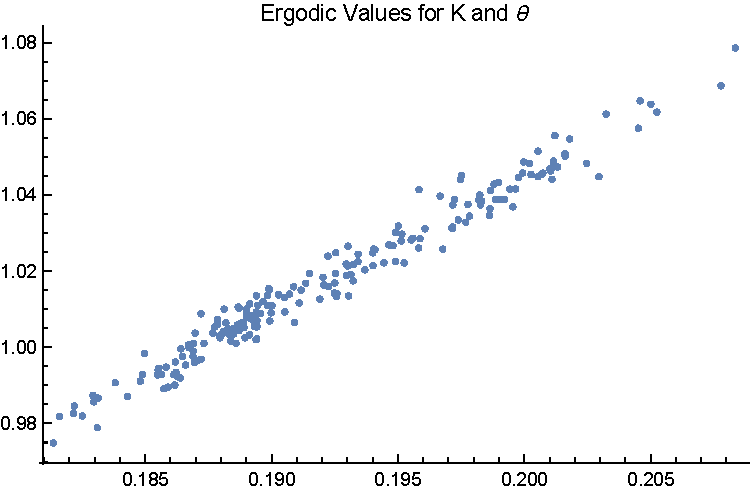
\includegraphics[width=2.5in]{ergodicKTheta.pdf}
  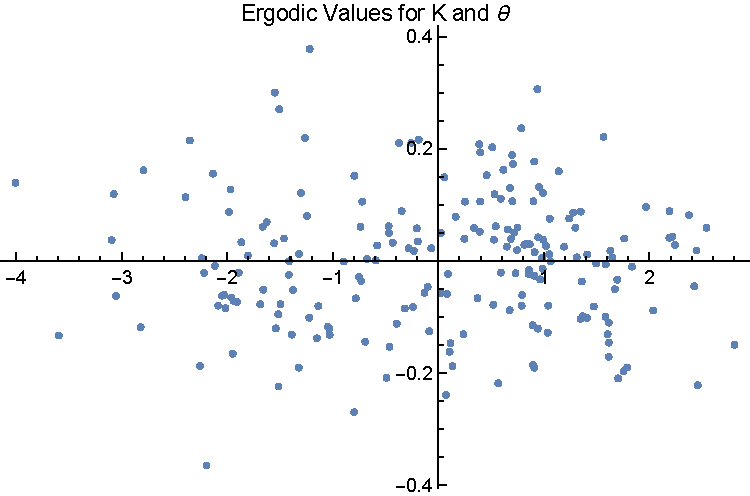
\includegraphics[width=2.5in]{ergodicZs.pdf}
  \caption{The Ergodic Values for $k_t, \theta_t$ }
  \label{fig:erg}
\end{figure}


\begin{gather}
\bar{X}= \vcenter{\hbox{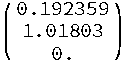
\includegraphics{ergodicMean.pdf}}}
\end{gather}
\begin{gather}
\sigma_{X}= \vcenter{\hbox{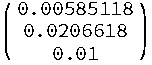
\includegraphics{ergodicSD.pdf}}}
\end{gather}


\begin{gather}
V= \vcenter{\hbox{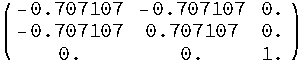
\includegraphics{ergodicV.pdf}}}
\end{gather}

\begin{gather}
\max Z= \vcenter{\hbox{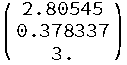
\includegraphics{ergodicMaxZ.pdf}}}
\end{gather}
\begin{gather}
\min Z= \vcenter{\hbox{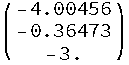
\includegraphics{ergodicMinZ.pdf}}}
\end{gather}


In what follows I show the impact of increasing the number of terms in the 
employed in the series representation.  
The figures  show contour plots for the norm of the error 
$\sqrt{(c_t-c_t^\star)^2 +(k_t-k_t^\star)^2 +(\theta_t-\theta_t^\star)^2 +(N_t-N_t^\star)^2 }$ for the approximated decision rule. The green dot shows the values of $(y_1,y_2)$ associated with the largest actual error.  The orange dot shows $(y_1,y_2)$ associated with  the largest equation system discrepancy 
that was used in computing the error bound. The black dots show the interpolation points. The label of the figure provides the predicted error bound along with the largest error.


Figure \ref{fig:cntpltA} shows the results when $K=0$, with degree of approximation $(1,1,1)$, the standard approach
for computing the decision rule.  The top panel provides a contour plot of the
norm of the equation errors. The bottom plot shows the error in the decision rule for different values of $k_{t-1}, \theta_{t-1}$ with $\epsilon_t=0$.  The plots for different values of $\epsilon_t$ are not different. The error bound, 
\ifmacosx
\input{resDir/forBetterRBC--1,1,1-Iters20theK0numKern2errBnd.tex} 
\fi
\iflinux
\input{resDir/forBetterRBC--1,1,1-Iters20theK0numKern0errBnd.tex} 
\fi
is 25\% larger than the actual error 
\ifmacosx
\input{resDir/forBetterRBC--1,1,1-Iters20theK0numKern2acterr.tex}
\fi
\iflinux
\input{resDir/forBetterRBC--1,1,1-Iters20theK0numKern16acterr.tex}
\fi
\begin{figure}
  \centering
\ifmacosx
  \includegraphics{resDir/forBetterRBC--1,1,1-Iters20theK0numKern2Approx.pdf}
  \includegraphics{resDir/forBetterRBC--1,1,1-Iters20theK0numKern2.pdf}
\fi
\iflinux
\includegraphics{resDir/forBetterRBC--1,1,1-Iters20theK0numKern16Approx.pdf}
\fi
  \caption{Contour Plot for approx=(1,1,1) K =0 (Standard Approach)}
  \label{fig:cntpltA}
\end{figure}

The panels in Figure \ref{fig:cntpltB} shows the results when $K=1,2,3,4,5$
while Figure



\begin{figure}
  \centering
\iflinux
\includegraphics[width=1.0in]{resDir/forBetterRBC--1,1,1-Iters30theK1numKern16.pdf}
\includegraphics[width=1.0in]{resDir/forBetterRBC--1,1,1-Iters30theK2numKern16.pdf}
\includegraphics[width=1.0in]{resDir/forBetterRBC--1,1,1-Iters30theK3numKern16.pdf}
\includegraphics[width=1.0in]{resDir/forBetterRBC--1,1,1-Iters30theK4numKern16.pdf}
\includegraphics[width=1.0in]{resDir/forBetterRBC--1,1,1-Iters30theK5numKern16.pdf}
\fi
\ifmacosx
\includegraphics[width=1.0in]{resDir/forBetterRBC--1,1,1-Iters20theK1numKern2.pdf}
\includegraphics[width=1.0in]{resDir/forBetterRBC--1,1,1-Iters20theK2numKern2.pdf}
\includegraphics[width=1.0in]{resDir/forBetterRBC--1,1,1-Iters20theK3numKern2.pdf}
\includegraphics[width=1.0in]{resDir/forBetterRBC--1,1,1-Iters20theK4numKern2.pdf}
\includegraphics[width=1.0in]{resDir/forBetterRBC--1,1,1-Iters20theK5numKern2.pdf}
\fi
  \caption{Contour Plot for approx=(1,1,1)  K =1,2,3,4,5}
  \label{fig:cntpltB}
\end{figure}



Figure \ref{fig:cntpltC} shows the results when $K=10$, with degree of approximation $(1,1,1)$
for computing the decision rule.  The top panel provides a contour plot of the
norm of the equation errors. The bottom plot shows the error in the decision rule for different values of $k_{t-1}, \theta_{t-1}$ with $\epsilon_t=0$.  The plots for different values of $\epsilon_t$ are not different.  The error bound, 
\ifmacosx
\input{resDir/forBetterRBC--1,1,1-Iters20theK10numKern2errBnd.tex} 
\fi
is 25\% larger than the actual error 
\iflinux
\input{resDir/forBetterRBC--1,1,1-Iters20theK10numKern111acterr.tex} 
\fi
 Notice that even though equation errors are comparable in magnitude, the error in the decision rule is significantly smaller for the series representation solution.  The additional constraints on the equation system provided by computing conditional expectations paths and incorporating them into the solution at time $t$ leads to better solutions.



\begin{figure}
  \centering
\iflinux
  \includegraphics{resDir/forBetterRBC--1,1,1-Iters20theK10numKern16Approx.pdf}
  \includegraphics{resDir/forBetterRBC--1,1,1-Iters20theK10numKern16.pdf}
\fi
\ifmacosx
  \includegraphics{resDir/forBetterRBC--1,1,1-Iters20theK10numKern2Approx.pdf}
  \includegraphics{resDir/forBetterRBC--1,1,1-Iters20theK10numKern2.pdf}
\fi
  \caption{Contour Plot for approx=(1,1,1) iters 20 K =10}
  \label{fig:cntpltC}
\end{figure}

\begin{figure}
  \centering
\iflinux  
\includegraphics{resDir/forBetterRBC--2,2,2-Iters20theK0numKern5.pdf}
\fi
\ifmacosx  
\includegraphics{resDir/forBetterRBC--2,2,2-Iters20theK0numKern2.pdf}
\fi
  \caption{Contour Plot for approx=(2,2,2) 20 iterations and K =0}
  \label{fig:cntpltD}
\end{figure}

\begin{figure}
  \centering
\iflinux
  \includegraphics{resDir/forBetterRBC--2,2,2-Iters20theK5numKern5.pdf}
\fi
\ifmacosx  
\includegraphics{resDir/forBetterRBC--2,2,2-Iters20theK5numKern2.pdf}
\fi
  \caption{Contour Plot for approx=(2,2,2) 20 iterations and K =5}
  \label{fig:cntpltE}
\end{figure}

\begin{figure}
  \centering
\ifmacosx
  \includegraphics{resDir/forBetterRBC--2,2,2-Iters20theK10numKern2.pdf}
\fi
  \caption{Contour Plot for approx=(2,2,2) 20 iterations and K =10}
  \label{fig:cntpltF}
\end{figure}

\begin{figure}
  \centering
\ifmacosx
  \includegraphics{resDir/forBetterRBC--2,2,2-Iters20theK20numKern2.pdf}
\fi
  \caption{Contour Plot for approx=(2,2,2) 20 iterations and K =20}
  \label{fig:cntpltG}
\end{figure}

\begin{figure}
  \centering
\ifmacosx
  \includegraphics{resDir/forBetterRBC--3,3,3-Iters20theK0numKern2.pdf}
\fi
  \caption{Contour Plot for approx=(3,3,3) 20 iterations and K =0}
  \label{fig:cntpltH}
\end{figure}

\begin{figure}
  \centering
\ifmacosx
  \includegraphics{resDir/forBetterRBC--3,3,3-Iters20theK10numKern2.pdf}
  \fi
  \caption{Contour Plot for approx=(3,3,3) 20 iterations and K =10}
  \label{fig:cntpltI}
\end{figure}

\begin{figure}
  \centering
\ifmacosx
  \includegraphics{resDir/forBetterRBC--3,3,3-Iters20theK20numKern2.pdf}
  \fi
  \caption{Contour Plot for approx=(3,3,3) 20 iterations and K =20}
  \label{fig:cntpltI}
\end{figure}
\subsubsection{Approximating an Unknown Solution: $U(c) \ne Log(c)$ }
\label{sec:unknown-solutions}

The algorithm we have described,
uses a proposed deterministic map
characterizing the evolution of expected values for
the dynamic system going forward. It then solves
a deterministic problem at time t to improve the proposed solution.
There is nothing in the algorithm that precludes accommodating  inequality
constraints.\footnote{See section \ref{sec:regime-switch-model} characterizing
  models with regime switching.} 
The algorithm we have described,
uses a proposed deterministic map
characterizing the evolution of expected values for
the dynamic system going forward. It then solves
a deterministic problem at time t to improve the proposed solution.
There is nothing in the algorithm that precludes accommodating  inequality
constraints.\footnote{See section \ref{sec:regime-switch-model} characterizing
  models with regime switching.}


\section{Future Work}
\label{sec:future}

\begin{itemize}
\item parallelMap don't need order, so ParallelTry  four args pretest posttest xvals keep all except failed  be sure to fail conflicts
\end{itemize}

\begin{description}
\item[Support Vector Machine Regression (SVMR)] By using SVMR to represent the solutions in place of Smolyak interpolation, a by product of the representation is the identification of influential points.  It should be possible to improve the algorithm performance by updating solutions only at these influential points.
\item[Large Model Implementation] It should prove useful to further exploit 
the high degree of parallelism available in the algorithm.
\item[Dynare Interface] 
\item[Improve Error Bounds] 
\end{description}
\section{Conclusions}
\begin{description}
\item[\href{https://github.com/es335mathwiz/AMASeriesRepresentation.git}{github access}] 
\end{description}
\label{sec:conc}




\bibliographystyle{plainnat}
\bibliography{anderson,files}
\appendix


\section{RBC Example}
\label{sec:rbc-example-1}

  We consider a model described in \cite{Maliar2005}\footnote{Here, we set their $\beta=1$ do not discuss quasi-geometric discounting or time-inconsistency.}
 \begin{gather*}
   \max\left \{  u(c_t) + E_t \sum_{t=0}^\infty  \delta^{t+1}u(c_{t+1})\right \}\\
c_t + k_t=(1-d)k_{t-1} + \theta_t f(k_{t-1})\\
f(k_t)= k_t^\alpha\\
u(c)=\frac{c^{1-\eta}-1}{1-\eta}\\
 \mathbb{L}= \left \{ 
 u(c_t)+E_t\sum_{t=0}^\infty \delta^{t}u(c_{t+1}) 
 \right \}+ \\
\sum_{t=0}^\infty 
\left \{ \delta^t \lambda_t  (c_t + k_t-((1-d)k_{t-1} + \theta_t f(k_{t-1}))) + \right . \\ 
\left . \delta^t \mu_t( (k_t - (1-d)k_{t-1} ) - \upsilon I_{ss})  \right \} \intertext{ so that we can impose}
 I_t =(k_t - (1-d)k_{t-1} ) \ge  \upsilon I_{ss}\intertext{ The first order conditions become}
\frac{1}{c_t^\eta} + \lambda_t\\
\lambda_t + \delta \lambda_{t+1}\theta_{t+1} \alpha k_t^{(\alpha-1)}+ \delta(1-d) \lambda_{t+1} + \mu_t + \delta (1-d)\mu_{t+1}
% \intertext{To computed the bordered Hessian we need}
% \nabla G_1=\nabla
% \begin{bmatrix}
% (c_t + k_t-((1-d)k_{t-1} + \theta_t f(k_{t-1})))\\
% -(c_t + k_t-((1-d)k_{t-1} + \theta_t f(k_{t-1})))\\
% (c_{t+1} + k_{t+1}-((1-d)k_{t} + \theta_{t+1} f(k_{t})))\\
% -(c_{t+1} + k_{t+1}-((1-d)k_{t} + \theta_{t+1} f(k_{t})))
% \end{bmatrix}=\\
% \begin{bmatrix}
%   1&1\\
%   -1&-1\\
% 0&(1-d)+\theta_{t+1}\alpha k_t^{(\alpha-1)}\\
% 0&-((1-d)+\theta_{t+1}\alpha k_t^{(\alpha-1)})
% \end{bmatrix}\\
% \nabla G_2=\nabla
% \begin{bmatrix}
% (c_t + k_t-((1-d)k_{t-1} + \theta_t f(k_{t-1})))\\
% -(c_t + k_t-((1-d)k_{t-1} + \theta_t f(k_{t-1})))\\
% (c_{t+1} + k_{t+1}-((1-d)k_{t} + \theta_{t+1} f(k_{t})))\\
% -(c_{t+1} + k_{t+1}-((1-d)k_{t} + \theta_{t+1} f(k_{t})))\\
% ( (k_t - (1-d)k_{t-1} ) - \upsilon I_{ss})\\
% ( (k_{t+1} - (1-d)k_{t} ) - \upsilon I_{ss})
% \end{bmatrix}
% \intertext{The second order conditions are}
% \begin{bmatrix}
% -\eta c^{-(\eta+1)}&0\\
% 0& \alpha(\alpha-1) k_t^{(\alpha-2)}
% \end{bmatrix}
\end{gather*}




\end{document}

